%%%%%%%%%%%%%%%%%%%%%%%%%%%%%%%%%%%%%%%%%%%%%%%%%%%%%%%%%%%%%%%
%
% Welcome to Overleaf --- just edit your LaTeX on the left,
% and we'll compile it for you on the right. If you open the
% 'Share' menu, you can invite other users to edit at the same
% time. See www.overleaf.com/learn for more info. Enjoy!
%
%%%%%%%%%%%%%%%%%%%%%%%%%%%%%%%%%%%%%%%%%%%%%%%%%%%%%%%%%%%%%%%

% ===============================================
% MATH 790: Real Analysis           Spring 2022
% hw_template.tex
% ===============================================

% -------------------------------------------------------------------------
% The preamble that follows can be ignored. Go on
% down to the section that says "START HERE" 
% -------------------------------------------------------------------------

\documentclass{article}

\usepackage[margin=1in]{geometry} 
\usepackage{amsmath,amsthm,amssymb,hyperref}
\usepackage{graphicx}
\usepackage{float}

\newcommand{\R}{\mathbf{R}}  
\newcommand{\Z}{\mathbf{Z}}
\newcommand{\N}{\mathbf{N}}
\newcommand{\Q}{\mathbf{Q}}

\newenvironment{theorem}[2][Theorem]{\begin{trivlist}
\item[\hskip \labelsep {\bfseries #1}\hskip \labelsep {\bfseries #2.}]}{\end{trivlist}}
\newenvironment{lemma}[2][Lemma]{\begin{trivlist}
\item[\hskip \labelsep {\bfseries #1}\hskip \labelsep {\bfseries #2.}]}{\end{trivlist}}
\newenvironment{exercise}[2][Exercise]{\begin{trivlist}
\item[\hskip \labelsep {\bfseries #1}\hskip \labelsep {\bfseries #2.}]}{\end{trivlist}}
\newenvironment{problem}[2][Problem]{\begin{trivlist}
\item[\hskip \labelsep {\bfseries #1}\hskip \labelsep {\bfseries #2.}]}{\end{trivlist}}
\newenvironment{question}[2][Question]{\begin{trivlist}
\item[\hskip \labelsep {\bfseries #1}\hskip \labelsep {\bfseries #2.}]}{\end{trivlist}}
\newenvironment{corollary}[2][Corollary]{\begin{trivlist}
\item[\hskip \labelsep {\bfseries #1}\hskip \labelsep {\bfseries #2.}]}{\end{trivlist}}

\newenvironment{solution}{\begin{proof}[Solution]}{\end{proof}}

\begin{document}

% ------------------------------------------ %
%                 START HERE                  %
% ------------------------------------------ %

\title{Computing in Communication Networks} % Replace with appropriate title
\author{Assignment \#4: Vehicular Scenario\\Vu Anh Minh Le} % Replace "Author's Name" with your name

\maketitle


\section{Running with docker}
\subsection{Running the server}
Pull the docker server by the command: \textbf{docker pull minhval0307/unitn\_gpstracking\_server:latest}
\\
Then run the command: \textbf{docker run -it --rm -d -p 8080:80 --name web minhval0307/unitn\_gpstracking\_server}
\\
On a web browser, access: \href{http://localhost:8080/}{http://localhost:8080/}
\\~\\
To stop the container, run: \textbf{docker stop web}
\subsection{Running the clients}
There are two kinds of clients, say CARS and DRONES.\\~\\
To run CARS client, run the following commands:\\
\textbf{docker pull minhval0307/publisher\_cars:latest}\\
\textbf{docker run -it --rm --name cars minhval0307/publisher\_cars}
\\~\\
To run DRONES client, run the following commands:\\
\textbf{docker pull minhval0307/publisher\_drones:latest}\\
\textbf{docker run -it --rm --name drones minhval0307/publisher\_drones}
\\~\\
To stop CARS and DRONES clients, run:\\
\textbf{docker stop cars drones}

\section{Running directly with application files}
Access \href{https://github.com/minhval/ComputingInComNet.git}{https://github.com/minhval/ComputingInComNet.git} to download the application source for both server and clients.\\~\\
Inside folder server/src, run \textbf{index.html} (by double clicking on it) to start the tracking page.
\\~\\
Inside folder clients/cars, run command \textbf{python3 publisher\_cars.py} to start CARS client.
\\~\\
Inside folder clients/drones, run command \textbf{python3 publisher\_drones.py} to start DRONES client.
\\~\\
Note: packages \textbf{numpy} and \textbf{paho-mqtt} must be installed before starting the clients.

\section{Images on the run}
Here are several images presenting the result after running the server and the clients.
\begin{figure}[H]
\centering
  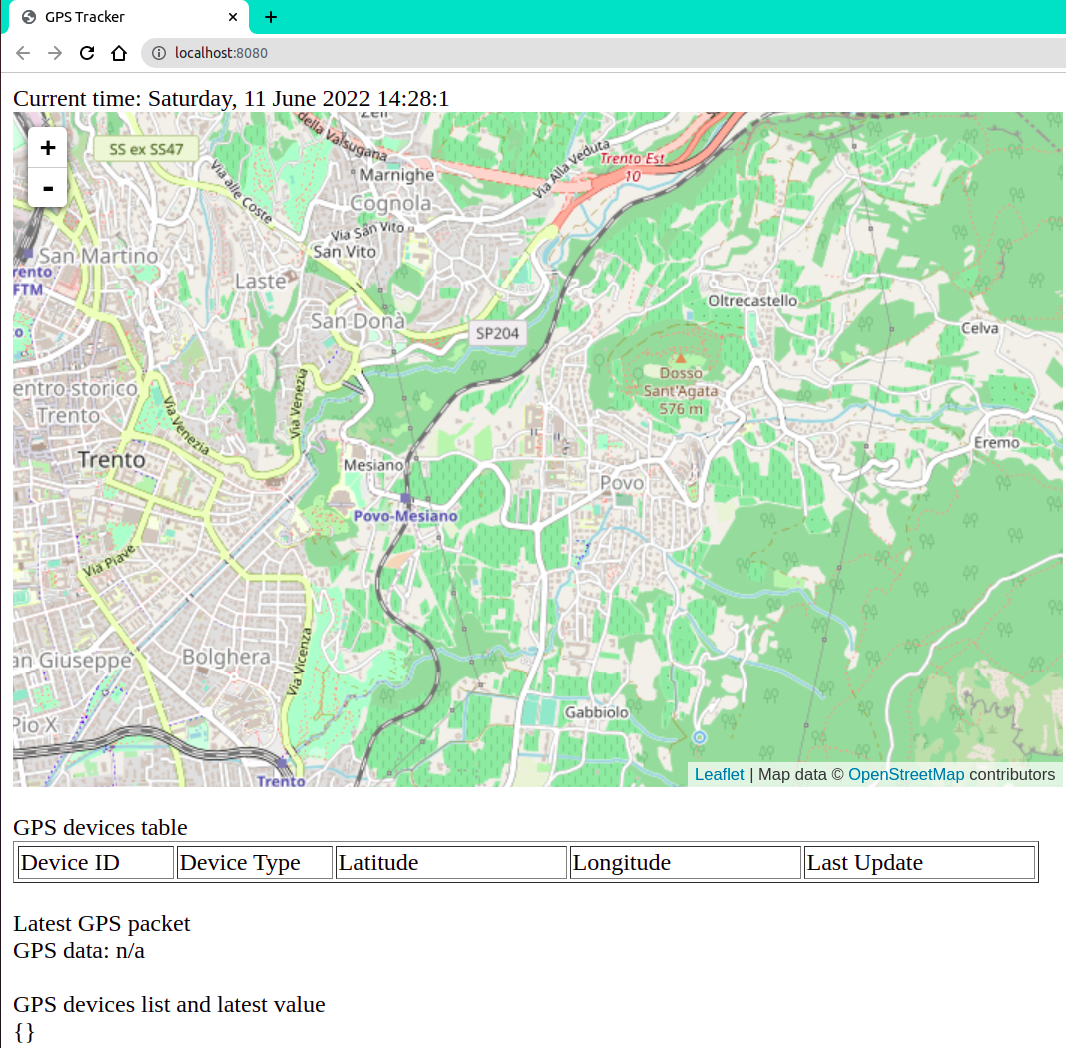
\includegraphics[width=1\textwidth]{fig/server.png}
  \caption{\textit{localhost:8080} with no data received.}
  \label{fig:server}
\end{figure}

\begin{figure}[H]
\centering
  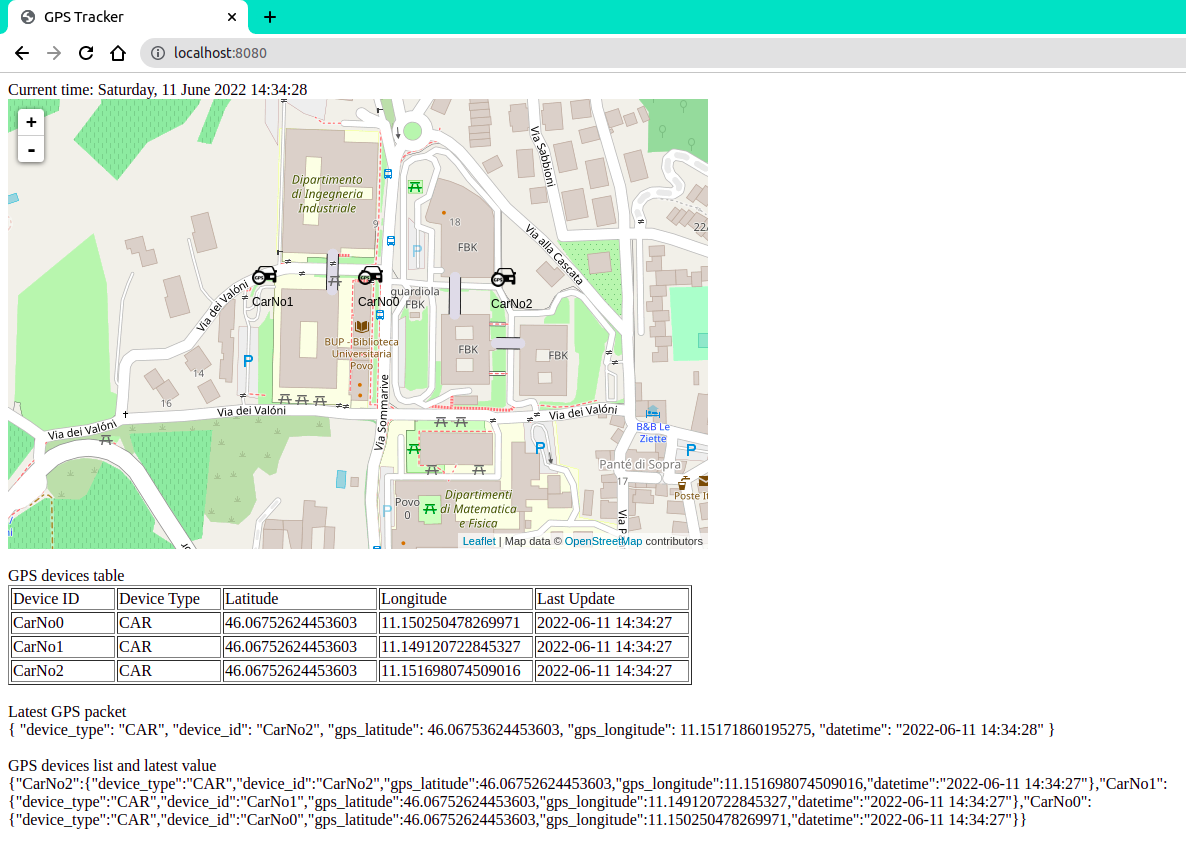
\includegraphics[width=1\textwidth]{fig/cars.png}
  \caption{\textit{localhost:8080} with CARS data after a while.}
  \label{fig:server}
\end{figure}

\begin{figure}[H]
\centering
  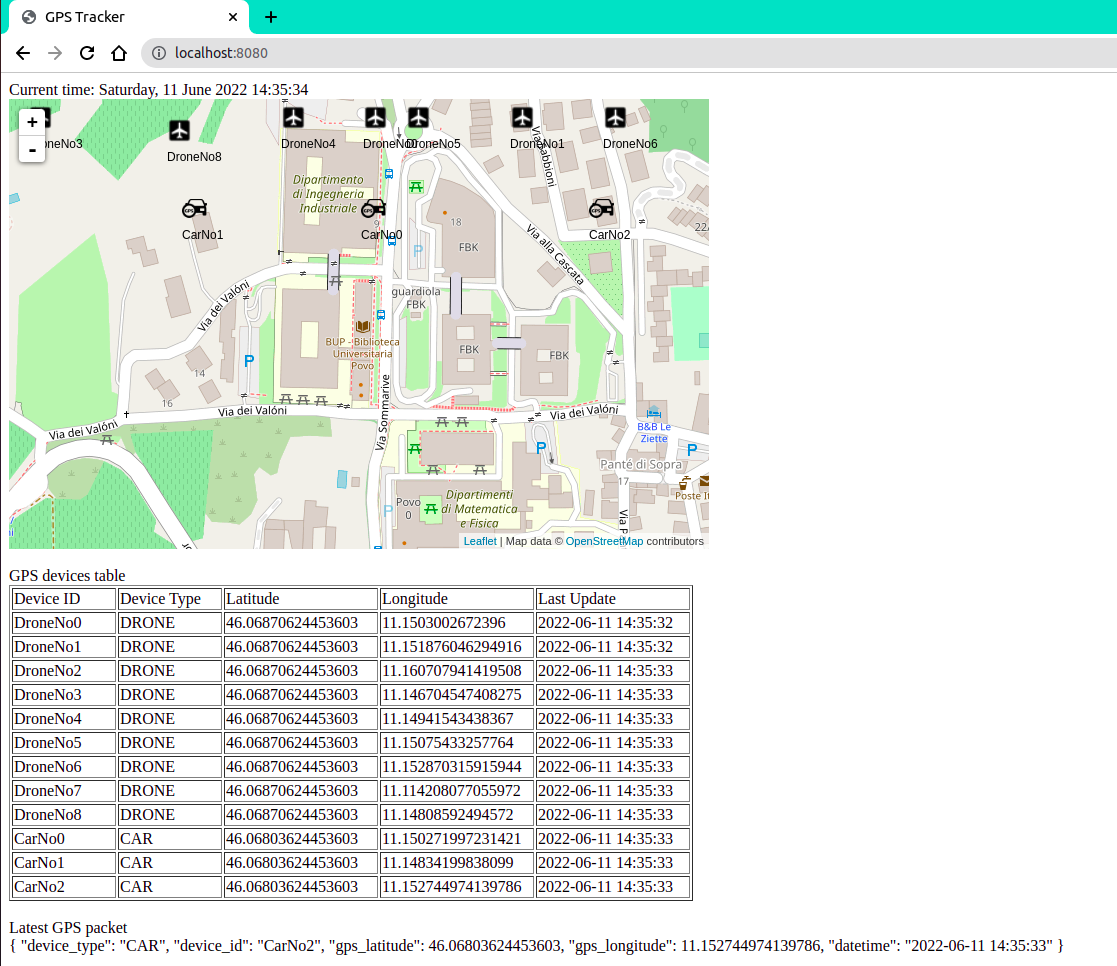
\includegraphics[width=1\textwidth]{fig/drones.png}
  \caption{\textit{localhost:8080} with CARS and DRONES data after a while.}
  \label{fig:server}
\end{figure}

\centering{
---

\end{document}